Dado este problema, encuentra la solución óptima entera mediante el algoritmo de Gomory de las formas enteras:

\begin{align*}
\max \quad & z = 3x_1 + 4x_2 \\
\text{s.a.} \quad & 2x_1 + 2x_2 \geq 1 \\
                  & 2x_1 + 2x_2 \leq 1.5 \\
                  & x_1, x_2  \in \mathbb{Z^+}
\end{align*}

Se ofrece esta solución factible habiendo aplicado el método de las dos fases:

\begin{center}
\begin{tabular}{c|c|cccc|}
 & $z$ & $x_1$ & $x_2$ & $h_1$ & $h_2$ \\ 
 & $-2.25$ & $0$ & $1$ & $0$ & $-3/4$  \\ 
\hline
$x_1$ & $3/4$ & $1$ & $1$ & $0$ & $1/4$ \\ 
$h_1$ & $1/2$ & $0$ & $0$ & $1$ & $1/2$ \\ 
\hline
\end{tabular}
\end{center}

---

Aplicando el método del Simple a la solución indicada, se llega a la solución óptima (no entera) cuya matriz completa es: 

\begin{center}
\begin{tabular}{c|c|cccc|}
 & $z$ & $x_1$ & $x_2$ & $h_1$ & $h_2$ \\ 
 & $-3$ & $-1$ & $0$ & $0$ & $-1$  \\ 
\hline
$x_2$ & $3/4$ & $1$ & $1$ & $0$ & $1/4$ \\ 
$h_1$ & $1/2$ & $0$ & $0$ & $1$ & $1/2$ \\ 
\hline
\end{tabular}
\end{center}

Como ya se tiene la solución óptima de la relajación lineal, se puede añadir el plano de corte $\frac{1}{4} h_2 \geq \frac{3}{4}$. No tiene sentido intentar hacer $h_1$ entera (no se indica en las restricciones de dominio del problema entero). La tabla se modificaría con la nueva restricción:
\begin{center}
\begin{tabular}{c|c|ccccc|}
 & $z$ & $x_1$ & $x_2$ & $h_1$ & $h_2$ &  $h^c_1$\\ 
 & $-3$ & $-1$ & $0$ & $0$ & $-1$  & $0$ \\ 
\hline
$x_2$ & $3/4$ & $1$ & $1$ & $0$ & $1/4$ & $0$\\ 
$h_1$ & $1/2$ & $0$ & $0$ & $1$ & $1/2$ & $0$\\ 
$h^c_1$ & -3/4&0&0&0&-1/4&1\\
\hline
\end{tabular}
\end{center}

La solución es no factible y cumple el criterio de optimalidad, luego entra en la base $h_2$ y sale $h^c_1$:


\begin{center}
\begin{tabular}{c|c|ccccc|}
 & $z$ & $x_1$ & $x_2$ & $h_1$ & $h_2$  & $h^c_1$ \\ 
 & $0$ & $-1$ & $0$ & $0$ & $0$ &  $-4$ \\ 
\hline
$x_2$ & $0$ & $1$ & $1$ & $0$ & $0$  & $1$ \\ 
$h_1$ & $-1$ & $0$ & $0$ & $1$ & $0$  & $2$ \\ 
$h2$ & $3$ & $0$ & $0$ & $0$ & $1$ & $-4$ \\
\hline
\end{tabular}
\end{center}

La solución a la que se llega cumple el criterio de optimalidad, es no factible ($h_1=-1$). Como no hay tasas de sustitución negativas no se puede seguir aplicando Lemke. La solución es no factible.

Aplicando el algoritmo de Gomory se observa que NO existen soluciones enteras factibles. 

Extra:

Se puede ver porque la restricción $\frac{1}{4} h_2 \geq \frac{3}{4}$ equivale a $x_1 + x_2 \le \frac{-3}{4}$. 

Como se puede ver en el gráfico la solución $(0,0)$, solución óptima de la RL tras añadir el corte de Gomory, no cumple el corte que se acaba de añadir. También se podía ver, para comprobar, que no existe ninguna solución entera que sea factible.

\begin{figure}[h]
    \centering
    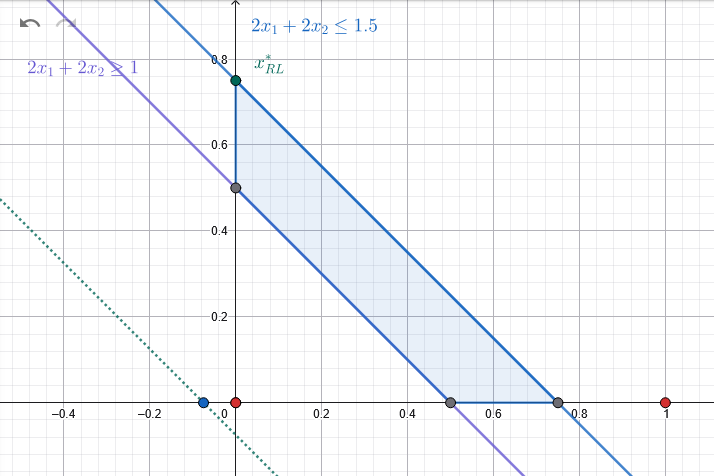
\includegraphics[width=0.5\textwidth]{ejercicios/gomory_entera_no_factible.png}
\end{figure}